%! TeX program = lualatex
\documentclass[../main.tex]{subfiles}
\begin{document} \section{Continuity and Non-differentiability}
  \begin{mdframed}[style=withref-compact] \label{thm:differentiability-implies-continuity}
    \textbf{Theorem}. If \(f\) is {differentiable} at \(a\), then \(f\) is {continuous} at \(a\).

    \textbook{Theorem 3.1 on page 237}
  \end{mdframed}

  \faComment{} If we know \(f(x)\) is continuous at \(a\), can we conclude that \(f(x)\) is also differentiable at \(a\)?
  \blanklines{5}

  \faComment{} What is the significance of Theorem~3.1? How do we use it?
  \blanklines{5}

  \begin{example}
    Explain why the following functions are not differentiable at \(0\).

    \begin{enumerate}[wide]
      \item \(g_{1}(x) = \frac{x - 1}{x}\).
        \blanklines{2}

      \item \(g_{2}(x) = \begin{cases} 1 &\text{if } x \ge 0 \\ 0 &\text{if } x < 0 \end{cases}\).
        \blanklines{2}

      \item \(g_{3}(x) = |x|\).
        \blanklines{3}

      \item \(g_{4}(x) = \sqrt[3]{x}\). 

        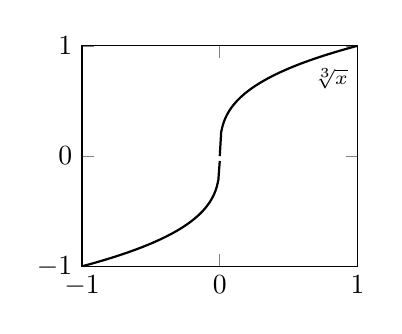
\begin{tikzpicture}
          \begin{axis}[samples=100, xmin=-1, xmax=1, ymin=-1, ymax=1, width={2in}, xtick={-1, 0, 1}, ytick={-1, 0, 1}]
            \addplot[thick, domain=0:1] {x^(1/3)};
            \addplot[thick, domain=-1:0] {-abs(x)^(1/3)};
            \node[left] at (1, 0.70) {\scriptsize \(\sqrt[3]{x}\)};
          \end{axis}
        \end{tikzpicture}
    \end{enumerate}
  \end{example}

  \clearpage

  % \begin{example}[Optional. Good practice for mathematical reasoning and problem-solving skill] \label{ex:differentiability-implies-continuity}
  %   \phantom{top}
  %
  %   Prove the theorem on page~\pageref{thm:differentiability-implies-continuity}. See the hint at the bottom of the page. 
  %
  %   \blanklines{40}
  %
  %   \begin{tikzpicture}[remember picture, overlay]
  %     \node[anchor=north, rotate={pi}, inner sep=0pt] at (current page text area.south) {\parbox{\linewidth}{\scriptsize 
  %           Hint to Example~\ref{ex:differentiability-implies-continuity}. By the limit laws, \(\lim_{x \to a} f(x) = f(a)\) is equivalent to \(\lim_{x \to a} \big( f(x) - f(a) \big)\).
  %       }};
  %   \end{tikzpicture}
  % \end{example}


\end{document}

